\begin{frame}[fragile]{Manche Sprachen sind schwerer zu beschreiben als andere}
    Wenn wir unsere Grammatiken einschränken, können wir nicht mehr alle Sprachen beschreiben.
    \metroset{block=fill}
    \begin{exampleblock}{Beispiel}
        Mit der Einschränkung\\
        \emph{Alle Produktionsregeln müssen der Form \alert{A $\to$ a oder A $\to$ aB} entsprechen, wobei A, B $\in$ V und a $\in \Sigma$}.\\
        können wir Sprachen wie $L_1 = \{a^n \mid n \in \naturals\}$ beschreiben,\\ aber nicht mehr Sprachen wie $L_1 = \{a^nb^n \mid n \in \naturals\}$.\\
        \alert{Achtung:} ist $\emptyWord \in L$, ist auch $S\to\emptyWord$ erlaubt, sofern $S$ nicht auf der rechten Seite einer Produktion vorkommt.
    \end{exampleblock}
    $\leadsto$ Sprachen, die wir mit dieser starken Einschränkung beschreiben können, nennen wir \alert{\emph{regulär}} oder vom \alert{\emph{Typ 3}}.\\
    Es gibt weitere Typen $\leadsto$ Mehr dazu in der Vorlesung
\end{frame}

\begin{frame}[fragile]{Manche Sprachen sind schwerer zu beschreiben als andere}
    \begin{center}
        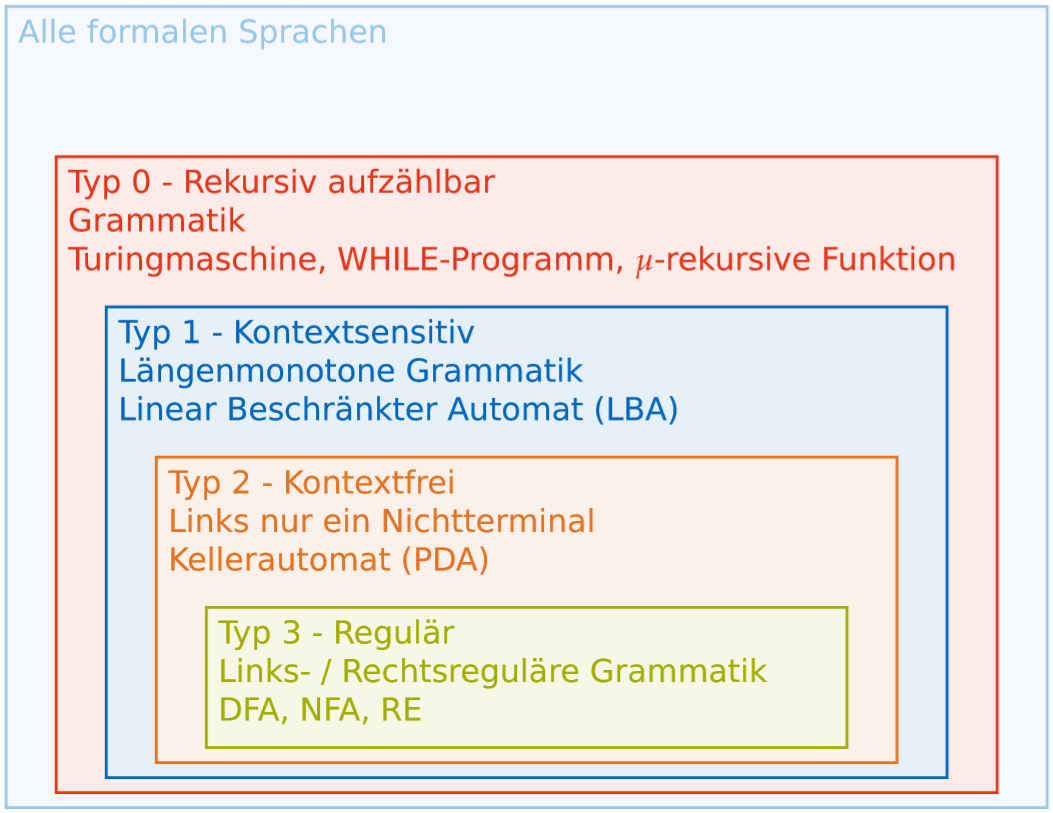
\includegraphics[width=0.75\textwidth]{../figures/Chomsky.png}
    \end{center}
\end{frame}

{\setbeamercolor{palette primary}{bg=ExColor}
\begin{frame}{Reguläre Grammatik}
    \begin{alertblock}{Aufgaben}
    Finde eine reguläre Grammatik für die folgenden Sprachen
    \end{alertblock}
    \metroset{block=fill}
    \begin{block}{Normal}
    \begin{itemize}
        \item $L_1 = \{a^{2n} \mid n\in\naturals\}$
        \item $L_2 = \{a^nb^m \mid n, m\in\naturals\}$
        \item $L_3 = \{uv \mid u\in\{a,b\}^\ast,\ v\in\{c,d\}\}$
        \item $L_4 = \{w \mid |w| = 3, w\in \{a,b,c\}^*\}$
    \end{itemize}
    \end{block}
    \begin{block}{Etwas Schwerer}
    \begin{itemize}
        \item $L_5 = \{a^n \mid n \equiv 1 \mod 3\}$
        \item $L_6 = \{uv\mid u\in\{\text{\Rewind, \MoveUp, \Forward, \MoveDown}\}^\ast,\;v\in\{\text{\Stopsign}\}\}$
        \item $L_7 = \{w \in \{a,b,c\}^* \mid |w|_a = 3, |w|_b = 1\}$
    \end{itemize}
    \end{block}
\end{frame}
}

{\setbeamercolor{palette primary}{bg=ExColor}
\begin{frame}{Lösung}
    \begin{itemize}
        \item<1-> \alert<1>{$P_1 = \{S \to aA \mid \emptyWord,\ A \to aB \mid a,\ B \to aA\}$}
        \item<2-> \alert<2>{$P_2 = \{S \to aA \mid bB \mid b \mid a \mid \emptyWord,\ A \to aA \mid bB \mid b \mid a ,\ B \to bB \mid b\}$}
        \item<3-> \alert<3>{$P_3 = \{S \to aS \mid bS \mid c \mid d\}$}
        \item<4-> \alert<4>{$P_4 = \{S \to aA \mid bA \mid cA,\ A \to aB \mid bB \mid cB,\ B \to a \mid b \mid c\}$}
        \item<5-> \alert<5>{$P_5 = \{S \to aA \mid a,\ A \to aB,\ B \to aS\}$}
        \item<6-> \alert<6>{$P_6 = \{S \to \text{\Rewind}S \mid \text{\MoveUp}S \mid \text{\Forward}S \mid \text{\MoveDown}S \mid \text{\Stopsign}\}$}
    \end{itemize}
\end{frame}
}

{\setbeamercolor{palette primary}{bg=ExColor}
\begin{frame}{Lösung}
        \begin{itemize}
            \item 
                \alert<1>{
                $P_7 = \{S \to cS \mid aA_1 \mid bB_0,$\\
                \vspace*{0.9mm}
                \hspace*{7mm}
                $\begin{aligned}
                A_1 &\to cA_1 \mid aA_2 \mid bB_1,\\
                A_2 &\to cA_2 \mid aA_3 \mid bB_2,\\
                A_3 &\to cA_3 \mid bB_3 \mid b,\\
                B_0 &\to cB_0 \mid aB_1,\\
                B_1 &\to cB_1 \mid aB_2,\\
                B_2 &\to cB_2 \mid aB_3 \mid a,\\
                B_3 &\to cB_3 \mid c\}
                \end{aligned}
                $}
        \end{itemize}
\end{frame}
}
